%
% fig-oberflaeche.tex
%
% (c) 2025 Prof Dr Andreas Müller
%
\begin{figure}
\centering
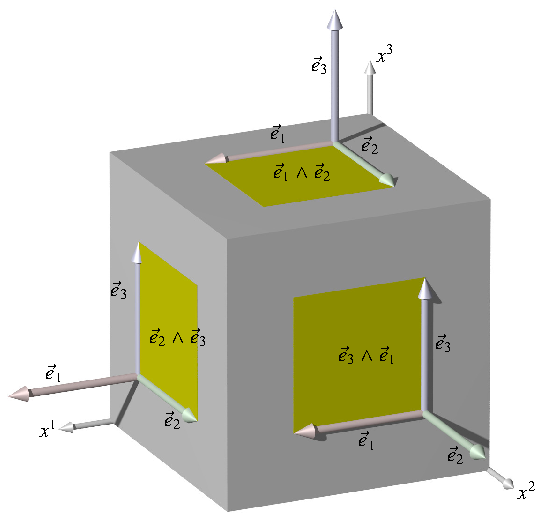
\includegraphics{chapters/050-gauss/images/oberflaeche.pdf}
\caption{Die Seitenflächen eines Koordinatenwürfels werden von den
Basis-2-Vektoren aufgespannt.
Für den Satz von Gauss müssen diese Seitenflächen untereinander kompatibel
orientiert sein.
Daher muss die von den Richtungen $\vec{e}_1$ und $\vec{e}_3$ aufgespannte
Seitenfläche die Orientierung von
$\vec{e}_3\wedge\vec{e}_1=-\vec{e_1}\wedge\vec{e_3}$
haben.
\label{buch:gauss:fig:oberflaeche}}
\end{figure}
